\documentclass[12pt,a4paper]{article}
\title{\Huge {Report}}
\author{Nicolas Kyejo}
\date{}

%%%%%%%%%%%%%%Declare PACKAGES%%%%%%%%%%%%%%%%%%

\usepackage{mathtools}  % or use \usepackage{amsmath}           
\DeclareMathSizes{12}{12}{8}{8}    %math font sizes
%\DeclareMathSizes{12}{20}{14}{10}  %try for size 12 text

%Uncomment the following for LaTeX helvetica clone
%\usepackage[utf8]{inputenc}
%\renewcommand{\familydefault}{\sfdefault} 
%\usepackage{helvet}

%Use XeLatex to render the following
%\usepackage{fontspec}
%\setromanfont[
%BoldFont=HelveticaLTStd-Blk.otf,
%ItalicFont=HelveticaLTStd-Light.otf,
%]{HelveticaLTStd-Roman.otf}


\usepackage[english]{babel}  %for labelling tables, graphics with english text. Use Finnish for finnish labelling
%\usepackage[official]{eurosym}	%euro symbol

%\usepackage{verbatim}      %for commenting huge blocks and dummy text
\usepackage{blindtext}

%Paragraph and Line spacing
\setlength{\parindent}{0pt}	%set paragraph indent to 0 points
\setlength{\parskip}{1em}  %spacing between paragraphs
\renewcommand{\baselinestretch}{1.5}    % set line spacing to 1.5

% Definition of \maketitle
\makeatletter         
\def\@maketitle{
\raggedright
%\includegraphics[width = 40mm]{logo.jpg}\\[8ex]
\begin{center}
{\Huge \bfseries \sffamily \@title }\\[4ex] 
{\LARGE  \@author}\\[4ex] 
{\large\@date}\\[8ex]
%\includegraphics[width=60mm]{metropolia-logo.png}    %logo in the title page
\end{center}}
\makeatother

\usepackage{graphicx}		%for putting pictures
\usepackage{float}            %for putting pictures at specified point

\usepackage{geometry} %Finnish document margins%
\geometry{
 a4paper,
 left=2cm,
 right=1.5cm,      %in reality has to 1cm
 top=1cm,
 bottom=2cm,
 }
 
\usepackage{fancyhdr}     %package for fancy header and footers
\usepackage{lastpage}     %records the last page number
\pagestyle{fancy}
\fancyhf{} % sets both header and footer to nothing
\renewcommand{\headrulewidth}{0pt}

% your new footer definitions here  
\cfoot{}
\lfoot{}
\rfoot{\thepage\ (\pageref{LastPage})}


\usepackage{hyperref}  		%for links
\hypersetup{colorlinks,breaklinks,
            urlcolor=[rgb]{0,0.5,0.5},    
            linkcolor=[rgb]{0,0.5,0.5}}    %set link color to Teal
            
\begin{document}
\maketitle
\thispagestyle{empty}      %remove numbering from bottom of this page
\newpage                   %page break
\tableofcontents
\thispagestyle{empty}      %remove numbering from bottom since pagestyle is empty
\clearpage
\newpage
\listoffigures
\thispagestyle{empty}      %remove numbering from bottom
\clearpage
\newpage
\setcounter{page}{1}        % set page counter from this page to 1

\section{Section 1}
\subsection{Subsection 1}
Static friction:
$$
F_{s_{max}} = \mu_s F_N
$$
where $F_{s_{max}}$ is the maximum static friction , $\mu_s$ is the coefficient of static friction and $F_N$ is the normal force perpendicular to the static friction force.

$$F_{s_{max}} = \mu_s F_N$$
$$\mu_s = F_{s_{max}}/F_N$$
$$    = F_{s_{max}}/9.8m $$where m is the mass of the load

$$ =  \frac{5.061 N}{0.7858 kg * 9.8 m/s^2} $$

$$ \mu_s = 0.65 $$

\subsection{Subsection 2}
\begin{figure}[H]
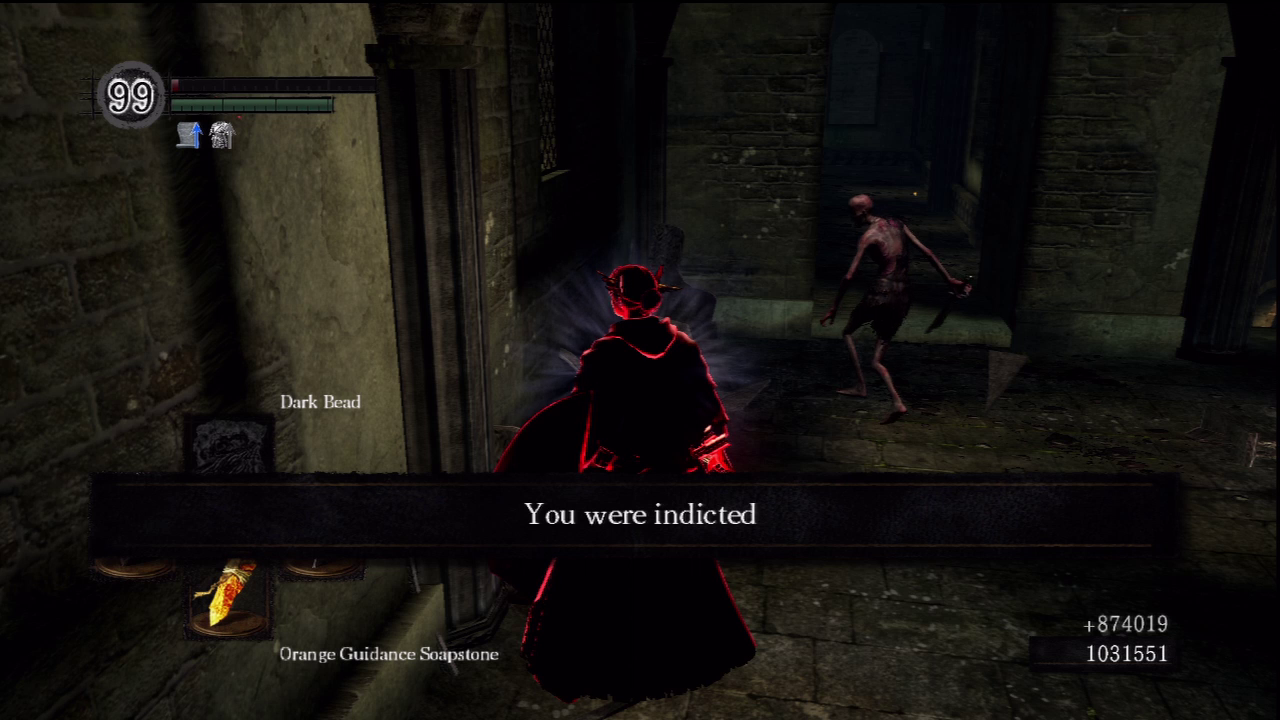
\includegraphics[width=\linewidth]{test}
\caption{\textit{Dark souls}}
\label{Indictment in dark souls} 
\end{figure}

\begin{table}[H]
\centering
\begin{tabular}{|c|c|}
\hline
\textbf{Range} & \textbf{Resolution} \\ 
\hline
$\pm$ 10 N	& 0.01 N \\
\hline
$\pm$ 50 N	& 0.05 N \\
\hline
\end{tabular} 
\caption{\textit{Simple table}}
\label{table:Force sensor resolution}
\end{table}

\section{Section 2}
\subsection{Subsection 1}
\paragraph{Definition of terms}
\begin{itemize}
\item Amplitude ($A$) is the difference in height from highest (maximum) to lowest (minimum) point divided by 2 within a single period ($T$). In other words, it is the function of the magnitude of the difference between the variables extreme values.
\item Period ($T$) denotes a single complete cycle of a periodic motion. Second ($s$) is the most common unit used.  $T = \frac{1}{f}$
\item Frequency $f$ describes how many times an event occurs in a single unit of time. In physics, frequency is most often applied to waves. It is denoted in Hertz $(Hz)$.  $f = 1/T$
\item Angular frequency $(\omega)$ measures angular displacement (radians) per unit time (seconds).
\item Kinematics of a periodic harmonic motion
	\begin{itemize}
	\item Displacement $(x), x = A sin(\omega t)$
	\item Velocity $(v), v = A\omega cos(\omega t), v = \pm \omega \sqrt{A^2-x^2}$
	\item Acceleration $(a), a = -A\omega^2 sin(\omega t)$
	\end{itemize}
\end{itemize}

\subsection{Subsection 2}
\blindtext

\end{document}
